%
%  Copyright © 2022 Mateusz Stompór. All rights reserved.
%

\chapter{Przegląd dostępnych rozwiązań}
Rozumiejąc główne idee stojące za generowaniem grafiki trójwymiarowej możliwe jest dalsze zgłębienie gałęzki informatyki odnoszącej się do tego zagadnienia.
Na przestrzeni lat powstał niemały zasób literatury poruszający tematykę.
Rozwiązania - silniki - będące implementacją idei rozwinięto do tego stopnia, że same w sobie nie są już komponentami aplikacji, ale wyewoluowały do samodzielnych, pełnoprawnych produktów.
Choć realizowane cele wydają się być identyczne - tworzenie obrazu na podstawie opisu sceny - to podejścia, które stosują różnią się znacząco od siebie.
Podobnie odmienne są wykorzystywane technologie.
Dotytyczy to zarówno programowania samej aplikacji, jak i komunikacji z GPU.
Celem niniejszego rozdziału będzie przegląd rozwiązań dostępnych na rynku, zestawienie ich ze sobą i analiza możliwości platform ekosystemu Apple.
\section{Materiały źródłowe}
Mając na uwadze współczesne trendy - potęgowanie informacji na skutek globalizacji i faktu iż każdy jest w stanie stworzyć publikacje - nie sam dostęp do informacji stanowi problem, a wartościowość źródeł.
Dokonująć przeglądu dostępnej literatury wyraźnie dostrzec można, że szczególną popularnością wśród obiorców cieszą się książki.
Ponadto, równie dużym zainteresowaniem i wkładem w rozwój dziedziny pochwalić mogą się publikacje pracowników firm z branży filmowej oraz gier.
Nie są to jednak jedyne kanały dostępne dla współczesnego odbiorcy.
Ostatnie piętnastolecie zaowocowało intensywnym rozwojem platform streamingowych.
Możliwość ta nie tylko pozwoliła zaangażować się twórcom niezaleznym, ale włączyła także instytucje, takie jak uczelnie.
Zainteresowani mogą bezpłatnie skorzystać z nagrań cyklów wykładów, które niegdyś zarezerwowany były tylko dla nielicznych.
\par
Źródła dostępne w formie książek podzielić można na kilka głównych kategorii - jest to literatura poświęcona odpowiednio: matematyce w świecie grafiki oraz implementacji algorytmów, śledzeniu promieni, a także projektowaniu i budowie silników do gier.
Nie można zapomnieć o narzędziach które konieczne są do rozwoju technologii - w tym kontekście odnosi się to do języków programowania w których technologie są tworzone - API programistycznych oraz środowisk na których są uruchamiane, takich jak systemy macOS, iOS, Windows, Linux.
\par
Pierwszą groupę, rozważającą aparat matematyczny oraz algorytmy wykorzystywane w generowaniu grafiki, reprezentują takie tytuły jak \textit{3D Math Primer for Graphics and Game Development}~\cite{math_f_dunn_i_parberry}, \textit{Real-Time Rendering}~\cite{real_time_rendering}.
Dostępne są one od wielu lat, posiadają szereg wydań i nieprzerwanie górują w wynikach sprzedaży na platformach takich jak eBay czy Amazon.
Choć statystyki sprzedaży nie muszą wiązać się z jakością samego dzieła to wartość wspomnianych tytułów podparta jest mnogimi referencjami w bibliografiach publikacji naukowych.
Obie pozycje skierowane są do osób posiadających niewielkie zaplecze inżynieryjne i stworzone przy założeniu, że czytelnik dopiero rozpoczyna zgłębianie tematyki.
Oba z dzieł przybliżają nomenklaturę używaną w branży, koncepcje przyjęte powrzechnie, opisują aparat matematyczny by w końcu przejść do właściwej części jaką jest renerowanie grafiki.
Mając szerszy ogląd nie sposób przeoczyć fakt, że pomimo ciągłej pracy ze strony autorów nie jest to odpowiednia literatura dla odbiorców poszukujących najświeższych nowinek.
Bezsprzecznie zagwarantować mogą silne podstawy i nakreślić idee, jednak chcąc stworzyć technologie aktualną należy odwołać się także do alternatyw.
\par
Warto pamiętać również o literaturze poruszającej kwestie rzucania promieni. 
Można przytoczyć tutaj między innymi \textit{Ray Tracing Gems}~\cite{ray_tracing_gems} oraz \textit{An Introduction to Ray Tracing}~\cite{ray_tracing_introduction}.
Zakres, który opisują jest znacznie szerszy niż współcześnie można wykorzystać w silniku czasu rzeczywistego, natomiast wiedza, która jest tam zawarta jest konieczna do uzyskania rozwiązania hybrydowego.
\par
Zrozumienie zasad generowania grafiki nie jest jednak wystarczająca do stworzenia biblioteki graficznej, ani bardziej obszernego wcielenia - silnika gry.
W tym celu należy zapoznać się z architekturą owocy branży rozrywkowej\cite{game_programming_patterns}.
Na rynku dostępne są produkcje stworzone wprost przez pracowników takich studiów jak \textit{Naughty Dog}\cite{game_engine_architecture} czy \textit{Electornic Arts}\cite{game_programming_patterns} opisujące problemy jakie twórcy mogą doświadczyć oraz propozycje ich rozwiązania.
Stonowi to nieodłączny suplement, ponieważ biblioteki graficzne czy też silniki gry mają za zadanie wyabstrahować skomplikowane techniki renderowania i zapewnić użytkownikowi środowisku w którym będzie w stanie realizować wizję artystyczną bez konieczności rozumienia o detale implementacyjne.
Jeśli chodzi o sam interfejs programistyczny trudno wytypować konkretne tytuły mogące pomóc w procesie projektowania.
Odwołać należy się do ogólnie przyjętych "dobrych" praktyk programistycznych, co w tym kontekście oznaczać może przejrzysty interfejs i możliwie dużą hermetyzację.
\par 
% Opisać też środowisko programistyczne XCode - będzie potrzebna ta wiedza w dalszej części pracy
Kolejnym ważnym elementem są źródła, które pozwalają przekuć idee związaniem z generowaniem grafiki w program komputerowy.
Z racji na platformę, oczekiwanie wysokiej wydajności wybór ogranicza się do języków takich jak Swift, Objective-C - natywnych dla macOS - oraz C++.
W przypadku C++ oraz Swift liczyć można na literaturę wprost od autorów \cite{cpp_bjorne}\cite{swift_docs}.
Objective-C choć stale wspierany i używany powszechnie nie jest już rozwijany i wachlarz dostępnych pozycji jest ograniczony. 
Pomimo tego pewne z nich zdecydowanie można uznać za solidne \cite{objective_c_kochan}. 
\par
Wprew intuicji w przypadku grafiki komputerowej badania publikowane przez uczelnie wyższe rzadko charakteryzują się innowacyjnością.
Zdecydowanie największy wkład we współczesny rozwój mają publikacje firm zaangażowanych bezpośrednio w dziedzinę z przyczyn komerycjnych.
Organizacje takie jak Crytek, Electronic Arts, Epic Games czy Ubisoft chętnie dzielą się informacjami związanymi z technikami renderowania i modelami oświetlenia.
Przykładami mogą być modele oświetlenia w silnikach \textit{Unreal Engine}~\cite{real_shading_ue_4} czy \textit{Frostbite}~\cite{moving_frostbite_to_pbr}.
Nie brakuje także przełomowych algorytmów, takich jak powszechnie używane \textit{SSAO}~\cite{finding_next_gen_cryengine2} stworzone przez Crytek czy \textit{mgła wolumetryczna}~\cite{volumetric_fog} przez Ubisoft.
Niezaprzeczalnie jednak w procesie tym przewodzą giganty takie jak Pixar czy Disney.
Nie tylko opisują oni jakie metody stosują, ale także tworzą sprawozdania podumowujące prace związane z konkretnymi produkcjami, ale także upubliczniają własne modele scen do mierzenia wydajności.
Zgodnie z tym co wspomniano na początku - wiedza z branży firmowej nie przkłada się bezpośrednio na ogólnie pojęte renderowanie czasu rzeczywistego - to jednak w obliczu układów tworzony współcześnie - wyposażonych w moduły akceleracji raytracingu - podejście to zyskuje na użyteczności.
\par
W ostatniej grupie źródeł - dystrybuowanych w formie materiałów wideo - umieścić można cykle wykładów z uczlni \textit{UC Davis}~\cite{uc_davis_computer_graphics}, \textit{MIT}~\cite{mit_computer_graphics} oraz \textit{Indian Institute of Technology Delhi}~\cite{iiotd_computer_graphics}. 
Są to kursy poruszające ogólną tematykę generowania obrazu.
Najaktualniejszy spośród nich należy do MIT - wykłady publikowane są corocznie.
Zrealizowane są one kompleksowo - zagadnienia są omówione szczegółowo, a w przypadku gdy wykraczają one poza przewidziany materiał prelegent informuje z jakiego zakresu należy wiedzę tę rozszerzyć.
Odbiorca więc nie będzie mógł posiąść wiedzy kompletnej na podstawie wideo, ale będzie wiedział jakie kierunki powinien zgłębić.
Pozostałe dwa kursy pomimo upłynięcia wielu lat od publikacji nadal są przydatne.
W szczególności \textit{Ken Joy} w ramach pracy w UC Davis opisuje dokładnie algorytmy wykorzystywane w sprzętowej akceleracji grafiki komputerowej.
Nie jest to wiedza niezbędna dla osoby chcącej zbudować silnik, ale pozwala zrozumieć w pełniej skali jak wygląda przebieg rasteryzacji.
\par
Równie użyteczne są wystąpienia pojedynczych osób - pracowników z branży gier - którzy opowiadają o podejściu, jakie należy stosować w celu uzyskania aplikacji o optymalnej wydajności.
Z uwagi na formę - zwykle jest to pojedynczy wykład nieprzekraczający godziny czasu - są one zwięzłe i jedynie nakreślają kierunek, jednak z racji iż branża gier potrzebuje najwyższej klasy wydajności to wzorce projektowe i podejście do programowania aplikacji niejednokrotnie budzi kontrowersje.
\par 
W przypadku platform Apple źródłem, które nie może być pominięte są wydarzenia WWDC~\cite{wwdc_conferences}.
Ich siłą jest możliwość zapoznania się z nowinkami technologicznymi, jakie twórcy udostępniają dla użytkowników swojego sprzętu.
Dodatkowo, często stanowią też okazję do skorygowania podejścia używanego przez programistów w celu zapewnienia optymalnej wydajności.
Przybierając przy tym formę zwięzłej prezentacji 20-60 minut wraz z dostarczeniem kodu źródłowego do samodzielnej analizy.
\par 
Ostatnimi, wartymi do przywołania źródłami są kanały w platformie youtube twórców niezależnych i pracowników korporacji zajmujących się produkcją gier.
Głównie wynika to z faktu, że pierwsi z nich są wyjątkowo otwarci na komentarz dotyczący technologii, które zastosowali i opisania krok, po kroku jak wygląda logika działania ich aplikacji.
Drudzy natomiast chętnie w formie dialogu z widzami przeprowadzają code-review lub też rozwijają wątki związane z tworzeniem silników.
Siła tej formy przekazu wynika z interaktywności.
Filmy same w sobie nie posiadają ograniczenia czasowego, nagrywający nie ponosi kosztów związanych z produkcją, ponieważ są one amatorskie, a sami widzowie mogą zadawać pytania, które adresowane mogą być w krótkim czasie.
\par
Podsumowując, Globalizacja, otwartość uczelni, a także korporacji sprawia, że dostęp do informacji nie stanowi żadnego problemu.
Dziedzina obfituje w wysokiej jakości źródła i wydaje się, że stworzenie rozwiązania bazującego na współczesnych trendach nie powinno stanowić wyzwania.
Problemem będzie natomiast nakład pracy potrzebny do uzyskania dzieła kompletnego pod względem funkcjonalnym oraz dobór technologii.
\clearpage
\section{Silniki 3D}
% Powinienem nakreślić że mamy rozwiązania multiplatformowe jak i te natywne.
% Wśród nich możemy wyróżnić silniki, które są open source, jak i te closed source.
% Dalej możemy określi te darmowe oraz te za które trzeba zapłacić 
% Opisać jak wygląda rozszerzalność tych rozwiązań
% Opisać jak wygląda wsparcie i dokumentacja
\subsection{Biblioteki multiplatformowe}
\subsubsection{Unity}
\begin{figure}[H]
    \begin{center}
        \includegraphics[width=10cm]{images/engines/unity/example-game.png}
    \end{center}
    \caption{Przykładowa gra stworzona w silniku Unity}
    \label{fig:unity-example-game}
\end{figure}

\subsubsection{Godot}
\begin{figure}[H]
    \begin{center}
        \includegraphics[width=15cm]{images/engines/godot/editor.png}
    \end{center}
    \caption{Edytor treści w silniku Godot}
    \label{fig:godot-editor}
\end{figure}

\subsubsection{Unreal Engine}
\fig{images/engines/ue/blueprints.png}{Kreator tworzenia logiki w silniku Unreal Engine 4}{fig:ue-blueprint}

\begin{figure}[H]
    \begin{center}
        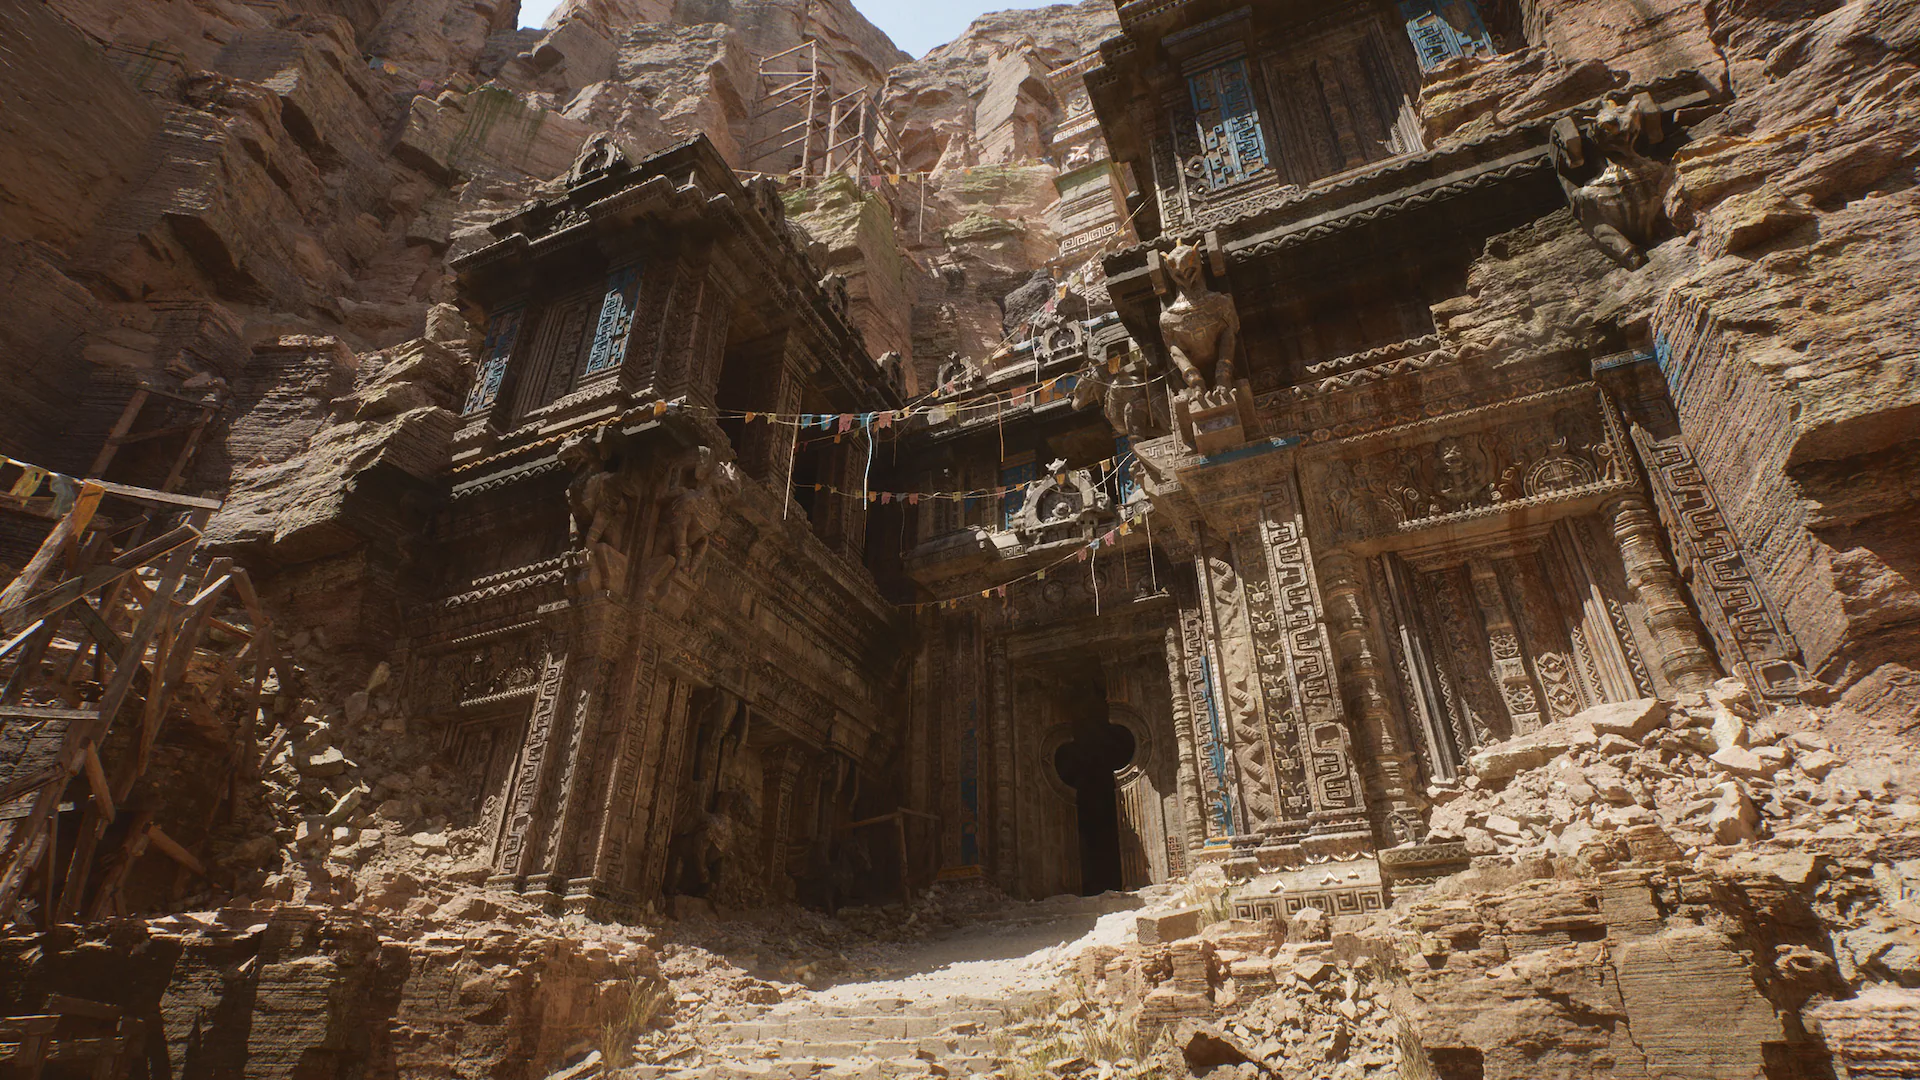
\includegraphics[width=15cm]{images/engines/ue/photorealistic-temple.png}
    \end{center}
    \caption{Przykład renderowania hybrydowego w Unreal Engine 5}
    \label{fig:ue5-photorealistic-temple}
\end{figure}

\subsubsection{Filament}
\begin{figure}[H]
    \begin{center}
        \includegraphics[width=7cm]{images/engines/filament/helmet.jpeg}
    \end{center}
    \caption{Przykład klatki wygenerowanej przez silnik Filament}
    \label{fig:filament-helmet}
\end{figure}

\subsection{Biblioteki natywne}
\subsubsection{SceneKit}
\begin{figure}[H]
    \begin{center}
        \includegraphics[width=15cm]{images/engines/scene-kit/editor.jpg}
    \end{center}
    \caption{Edytor treści w silniku SceneKit}
    \label{fig:scenekit-editor}
\end{figure}

\begin{figure}[H]
    \begin{center}
        \includegraphics[width=15cm]{images/engines/scene-kit/example-game.jpg}
    \end{center}
    \caption{Przykładowa gra w silniku SceneKit}
    \label{fig:scenekit-example-game}
\end{figure}
% Debiut rozwiązania nastąpił w 2012 roku. 
% Za projekt i wykonanie odpowiedzialna jest firma Apple, której urządzenia stanowią jedyną decelową grupę odbiorców oprogramowania.
% Początkowo wsparcie ograniczało się do platformy OS X, rozszerzenie dostępności na urządzenia mobilne została odroczone do 2014 roku.
% Kod źródłowy projektu nie jest dostępny publicznie, jednak uzyskanie dostępu do plików binarnych biblioteki jest darmowe.
% Nie podlega opłacie także wykorzystanie jej we własnym projekcie bez względu czy jego dalsza dystrubucja jest odpłatna.
\subsubsection{ARKit}

\begin{figure}[H]
    \begin{center}
        \includegraphics[width=15cm]{images/engines/ar-kit/example-app.jpg}
    \end{center}
    \caption{Rzeczywistość rozszerzona na przykładzie aplikacji mobilnej}
    \label{fig:arkit-example-app}
\end{figure}

% Tutaj mogę napisać, że to jest nowe wcielenie, które lepiej oddaje obecne podejście firmy do projektowania - nacisk na luźne powiązania, sprawienie, że
% osoby korzystające z biblioteki mają ułatwione testowanie

\subsection{Zestawienie}
\section{Języki programowania}
% Idea jest taka, żeby trochę "bezpłciowo" opowiedzieć o tych językach
% Pokazać dobre i słabe strony, bez sugestii, który zostanie wybrany
\subsection{C++}
\subsection{Swift}
\subsection{Objective-C}
\section{Interfejsy programistyczne}
\subsection{DirectX, OpenGL, Vulkan}
\subsection{Metal}
\subsection{Metal-C++}
\subsection{SPIRV}

